\documentclass[fontsize=11pt]{article}
\usepackage{amsmath}
\usepackage{float}
\usepackage[utf8]{inputenc}
\usepackage[margin=0.75in]{geometry}
\usepackage{tikz}
\usepackage{hyperref}
\usepackage[style=apa,backend=biber]{biblatex}
\addbibresource{bibliography.bib}


\title{CSC110 Project: A Study of Online Conspiracy Theories Regarding COVID-19}
\author{Aaron Ma, Benjamin Liu, Vishnu Nittoor}
\date{Friday, November 5, 2021}

\begin{document}

\maketitle

\section{Introduction}

\paragraph{Research Question} \textbf{What is the nature of the circulation and development of conspiracy theories surrounding COVID-19?}

\paragraph{Problem Description} Since the advent of the COVID-19, the world has witnessed the circulation and development of conspiracies surrounding the origin of the virus, the efficacy and nature of the new vaccines, and the political motivations behind COVID-related policy decisions. Although these conspiracy theories may be seemingly innocuous, they originate significant public unrest surrounding the vaccine, masking policies, the origins of COVID, and more.

We observe that the anti-mask movement, the anti-vaccine movement, and nationalistic narratives that suggest that the virus was engineered are key products of such conspiracy theories. Examples of certain ideas originated by these conspiracy theories involve the perception of COVID-19 as an attempt at biological warfare, that the vaccine causes and helps proliferate diseases such as autism, and that the pandemic was part of an elaborate business strategy for pharmaceutical firms to generate abnormal amounts of revenue.

Several accounts such as \cite{PeopleWh91:online} report that conspiracy theories severely impact the well-being of those that believe and spread them. Further, they pose emotional and physical risks for others around them - \cite{10.2307/27040260} suggests that ideologically diverse extremist groups who are especially reactive to these conspiracy theories, pose the threat of violent terrorism in the public domain. On a global scale, these theories have escalated political tensions, promoted anti-masking and anti-vaccination, and have acted against the dissemination of reliable information about the pandemic and the preventative measures that are relevant, according to \cite{COVID19c99:online}. 

We are motivated by these problems to investigate the bidirectional relationship between COVID-19 case data and conspiracies surrounding the pandemic.  Specifically, we would like to examine when these conspiracy theories gained prominence relative to the spread of the virus, how they are related in content to the pandemic, and how emotionally charged they are, and the popularity of certain topics over time.



\section{Dataset Descriptions}
\label{sec:dataset_descriptions}

We will be using two datasets for this dataset.
\begin{enumerate}
    \item \textbf{COVID-19 Case Dataset} We used COVID-19 case data provided by Our World In Data \cite{covid19d6:online}. Out of the many options given, we used the JSON file representing daily case data segregated by country (with a worldwide aggregate). We only used the worldwide aggregate of the daily case data. Other country-relevant statistics such as median age, population density, etc. was present, but ignored by our data aggregation function.
    
    We used the following fields for each entry in the dataset that represented one day's worth of cases:
    
    \begin{enumerate}
        \item The field \texttt{new\_cases}, an integer representing the number of new cases in the day
        \item The field \texttt{date}, a string formatted in \texttt{``YYYY-MM-DD''} representing the date corresponding to the dataset entry
    \end{enumerate}
    \item \textbf{Reddit Post Dataset From r/conspiracies} We are going to be investigating conspiracy theories surrounding COVID-19 using post data from the subreddit \cite{2conspir6:online}, a page on the popular message board/forum website Reddit. Being an incredibly active page with 1.6 million members, each post contains a title, a score representing net "upvotes" versus "downvotes", comments, and a text body. We will only consider text-based posts for this project. We will be extracting data from the subreddit using our own web scraping script.

    The data output of the script is a JSON file containing data that corresponds to a variety of attributes. The API used by the script is PushShift Reddit (API \cite{pushshif39:online}), which provides a large array of attributes for each post. Out of the several, we are only considering each post's title, number of comments, score, and the created time in seconds since the Unix epoch (detailed in \cite{Epoch0:online}).
    \item \textbf{1000 Most Commonly Used Words} This (\cite{deekayen_1000_nodate}) is a dataset of the 1000 most commonly used words in English. We require this dataset to filter out common words while performing frequency analysis on text in the Reddit posts when we are determining good keywords to search for.
\end{enumerate}

\section{Computational Overview}

\subsection{Major Computations}
\label{subsec:major_computations}

\paragraph{Data Collection}
    Since the COVID-19 case dataset is provided completely by Our World In Data, there is no additional dataset construction necessary for this portion of the data collection. A JSON file containing all the information we required was downloaded and stored in a subfolder \texttt{/data}. 
    
    The 1000 most commonly used words dataset is simply downloaded and renamed in order for our methods to later load the file into memory.
    
    For the dataset of Reddit posts, we designed a method (provided in the file \texttt{collect\_reddit\_data.py}) which was responsible for querying the PushShift API described in Section \ref{sec:dataset_descriptions}. After querying this API every second for the post data in a 5-day window (while filtering the query for the specific fields we are interested in), the method extended an accumulator list of all Reddit posts. Then, this list was written in JSON format to the file \texttt{pushshift-reddit-extracted.json} in the \texttt{/data} subfolder.
    
\paragraph{Data Aggregation}
    
    All data aggregation functions are enclosed in the file \texttt{data\_aggregation.py} in the parent directory. We constructed the dataclass \texttt{RedditObject} to store all relevant attributes of a Reddit Post (described in Section \ref{sec:dataset_descriptions}) for ease of access, and wrote functions to load the incoming Reddit data (stored after running the previous algorithm in a JSON file), clean the post title for uniformity in sentiment analysis, and load the COVID-19 data from the JSON file (only loading the worldwide cases into memory).
    
    In order to determine a good list of keywords and topics, we developed \texttt{freq\_analysis.py}. This file loads all Reddit posts, computes the number of times each word appears in the text, and then filters out the 1000 most commonly used words. Running the file prints the 100 most frequently used words on the subreddit (discounting the common English words that we filtered out). This part is essential for the data aggregation process - one of the main components in the data aggregation is assembling keywords and topics, all of which are detailed in the file \texttt{constants.py}.
    
\paragraph{Computational methods}

Our main computational methods are found in \texttt{computations.py} and are enumerated as follows: 

\begin{enumerate}
    \item We calculate the popularity of a post in \texttt{calculate\_popularity(post: RedditObject) -> int} by adding the post's score (net upvotes vs downvotes) to its number of comments.
    \item We calculate the degree of relation of a topic to a post in the function \texttt{calculate\_relation}. We scan for keywords in the post title and body, and return 1.0 if we find that one of the topic's keywords matches, and 0.0 if not. The motivation for returning a float is to allow for variability in the degree of relation between topics and posts in future iterations of the project.
    \item Arguably our \textbf{most important method}, the function \texttt{calculate\_sentiment\_from\_text} calculates the negative/positive of a Reddit post and returns a value between -0.5 and 0.5 representing this quantity. 
    
    Sentiment detection is done using a default sentiment classifier from the Python library flair \cite{akbik2019flair}, a library which describes itself as ``An easy-to-use framework for state-of-the-art NLP''. 
    
    Note that the confidence value given by the classifier represents the degree of confidence of a post being either negative or positive, and is bounded above by 1 and below by 0.5 - a lower confidence value would imply that the classifier is more confident in the other option, contradicting our assumption that the classifier reports the class in which it is most confident. So, we subtract 0.5 from this confidence value for continuity between our reported valences. We also give this value a sign depending on whether the sentiment is negative or positive. Therefore, our valence levels range from -0.5 to 0.5.
    
    The classifier is only loaded when it needs to be called; we use the Python library Joblib (\cite{joblib}) to cache our function results for inputs that we have encountered before, and we save this cache to the disk in the folder \texttt{'/cachedir'}. This is both for ease of development and for running the main sentiment analysis method without facing the large, repeated computational cost of recomputing the sentiments associated with the same text inputs.
    
    \textbf{NOTE: Despite PythonTA disallowing the use of nonconstant global variables, we found that it is required for us to have two nonconstant global variables representing the \text{Memory} and \text{TextClassifier} objects respectively} - any alternative implementation (that does not include major refactoring) includes loading the TextClassifier each time the function is called (and not caching our results) which would result in our running time increasing by a massive factor.
    
    \item We have the functions \texttt{posts\_in\_interval} and \texttt{new\_cases\_in\_interval} that filter the lists of posts and cases respectively to only contain those which are in the time interval specified. A similar function filters posts by topic: unsurprisingly, the function is named \texttt{filter\_posts\_by\_topic}.
    
    \item We calculate the total valence of posts in an interval in the function \texttt{calculate\_total\_valence} by summing the valences of all posts in the interval.
    
    \item The function \texttt{get\_time\_array} returns a one dimensional list containing timesteps between the beginning \texttt{start} and \texttt{end} timestamps, each spaced by the \texttt{resolution}, which is a \texttt{datetime.timedelta} object.
\end{enumerate}

\subsection{Computation and reporting of results}

We compute our results through various functions given in \texttt{main.py}. They are detailed as follows:

\begin{enumerate}
    \item The function \texttt{run\_popularity\_vs\_negatively\_charged} loads the Reddit posts, calculates popularities and sentiments for each post, and plots them on a scatter plot by calling the corresponding plotting function. We colour each post on the scatter plot according to its valence (a solid red represents completely negative, a solid green represents completely positive). 
    
    \item The function \texttt{run\_frequency\_over\_time} calculates the number of posts in intervals spaced a week apart each, starting 1st December 2019 and ending at the current date, and plots the number of posts per week over time by calling the corresponding plotting function. It also loads the COVID-19 case data, counts the number of new cases within the timeframe of a week at the relevant points in time, and plots this case frequency data alongside the post frequency over time. 
    
    \item The function \texttt{run\_valence\_over\_time} calculates the total valence of posts in intervals spaced a week apart each, starting 1st December 2019 and ending at the current date, and plots the total valence of posts in the week over time by calling the corresponding plotting function. It also loads the COVID-19 case data, counts the number of new cases within the timeframe of a week at the relevant points in time, and plots this case frequency data alongside the valence over time. 
    
    \item The function \texttt{overall\_valence\_histogram} plots the valence data of all posts on a histogram by calling the corresponding plotting function. The motivation of this function is to observe the distribution of the post valences over the interval from -0.5 to 0.5. 
    
    \item The function \texttt{run\_topics\_vs\_time} takes in a list of topics to track. Similar to the approach of the previous functions, it looks at posts within a timeframe of a week at different points in time, and calculates the aggregate relation of the relevant posts to a topic by summing outputs of the function \texttt{calculate\_relation} over the relevant posts. It also loads the COVID-19 case data, counts the number of new cases within the timeframe of a week at the relevant points in time, and plots this case frequency data alongside the total topic relation over time. The plotting is done by calling the corresponding plotting function.
    
    \item The functions \texttt{most\_negative\_posts} and \texttt{most\_positive\_posts} serve to print the 10 posts with the most extreme valence for our analysis. 
\end{enumerate}

% \subsection{Reporting Results}

% We will report results as follows, aiming to answer each of the below questions with a relevant figure that contains information on the variables in question.

% \begin{enumerate}
%   \item \textbf{Does the popularity of conspiracy theories depend on how negatively charged they are?}

%         We will plot post popularity against post intensity and use a polynomial regression model from the \texttt{numpy} library (using the function \texttt{numpy.polyfit} to calculate coefficients of the model and \texttt{numpy.polyval} to sample them for the figure).
%   \item \textbf{To what extent are COVID-19 conspiracy theories dependent on the proliferation of the virus?}

%         We will plot both post frequency and number of confirmed cases against time on parallel vertical axes. We will compute the Pearson correlation coefficient using \texttt{numpy.corrcoef}.
%   \item \textbf{What recurring topics of discussion develop over time amongst the conspiracy theories?}

%         We will plot multiple curves, each representing a topic class, against time. This, with a graph in parallel representing COVID-19 cases, would help determine the temporal relationship between key events in the pandemic and concurrent topics of discussion.
% \end{enumerate}

\subsection{New libraries used}

The most important new libraries that the project uses are as follows:

\begin{enumerate}
    \item \texttt{flair}
    
    This library (\cite{akbik2019flair}) powered our sentiment analysis; we were able to load a pre-existing text classifier using 
    
    \texttt{TextClassifier.load('en-sentiment')}, and then use this classifier to predict whether post titles were positive or negative. We also had to use the \texttt{Sentence} class to initialize a sentence containing our post title, on which we ran the \texttt{classifier.predict} method to obtain valence scores. More details on how these scores are used and transformed is given in Section \ref{subsec:major_computations}.
    
    \item \texttt{joblib}
    
    We used this library (\cite{joblib}) to cache the function results of \texttt{calculate\_sentiment\_from\_text} in order for ease of development and for running the main sentiment analysis method without facing the large, repeated computational cost of recomputing the sentiments associated with the same text inputs, as mentioned above. 
    
    We used the decorator \texttt{@memory.cache} above the function to indicate that we would like to cache the outputs of this function to disk, and specified the caching location while initializing an instance of the \texttt{Memory} object in the line \texttt{memory = Memory("cachedir")}.
    
    \item \texttt{requests}
    
    This library (\cite{noauthor_requests:_nodate}) was used in order to query the PushShift API given the r/conspiracies subreddit and the appropriate timeframe.
    \item \texttt{json}
    
    We used this library to load json files. The function \texttt{json.load} was used for this purpose.
    \item \texttt{matplotlib.pyplot}
    
    We used this library to do all of our plotting. The most critical functions used were \texttt{plt.plot} and \texttt{plt.scatter}.
\end{enumerate}

\section{Instructions}

The entire project repository is found at \href{https://github.com/nitvishn/csc110-project}{https://github.com/nitvishn/csc110-project}, if needed.

\subsection{Obtaining datasets}

To ensure that the datasets used by our TA are \textit{exactly} the ones we used, we will provide links to a GitHub repository on which our project is hosted. We will be submitting the file used to generate the extracted Reddit dataset, but we do not require the TA to execute this file to query the API and generate the dataset themselves.

\begin{enumerate}
    \item The COVID-19 dataset may be obtained by downloading \href{https://raw.githubusercontent.com/nitvishn/csc110-project/master/data/pushshift-reddit-extracted.json}{this JSON file} (hosted on our GitHub repository). It must be placed in a subfolder named \texttt{/data}.
    \item The Reddit post dataset may be obtained by downloading \href{https://raw.githubusercontent.com/nitvishn/csc110-project/master/data/owid-covid-data.json}{this JSON file} (hosted on our GitHub repository). It must be placed in a subfolder named \texttt{/data}.
    \item The commonly used words dataset may be obtained by downloading \href{https://raw.githubusercontent.com/nitvishn/csc110-project/master/data/commonly_used_words.txt}{this TXT file} hosted on our GitHub repository. It must be placed in a subfolder named \texttt{/data}.
\end{enumerate}

\subsection{Running the program}

It is important to create the empty directory \texttt{/figures} before running the program in order for the program to store all its visualizations correctly.

After installing all requirements given in \texttt{requirements.txt}, and after ensuring that the files 

\texttt{/data/pushshift-reddit-extracted.json}, \texttt{data/owid-covid-data.json}, and \texttt{data/commonly\_used\_words.json} are present, you may run \texttt{main.py}.

Expect the download of the flair text classification model for sentiments to take 2-5 minutes - once this file is downloaded, the model will be executed on all Reddit posts. On first run, logs will be printed by the \texttt{joblib} module indicating that the function outputs are being cached for \texttt{calculate\_sentiment\_from\_text}. 

The \textbf{main output} from our program is the set of images that represent the various figures that we plot our final results on. These figures will be present in the \texttt{/figures} directory after \texttt{main.py} terminates.

\section{Changes from proposal}
There were a few changes to the computational plan to the project. We have documented them below.
\begin{enumerate}
    \item The OSRSBox Reddit scraper did not obtain the date posted for each post, so we swapped it out for our own Reddit scraping script. This script is detailed in Section \ref{subsec:major_computations}.
    \item Our choices of keywords was not sufficient to categorize the majority of Reddit posts, so we instead performed a frequency analysis to determine our list of keywords.
    \item We initially assumed that the relationship between post sentiments and popularity would be modelled by a polynomial relationship - it is not. Instead, it is to our benefit to plot these on a scatter plot and intuitively analyze the behaviour of posts at the extremes. More information is present below in Section \ref{sec:discussion}.
    \item The VADER sentiment algorithm did not seem to effectively determine the sentiment of many Reddit posts - a lot of seemingly aggressive posts were classified as neutral. Instead, we used the \texttt{flair} library for sentiment analysis. More details are present in Section \ref{subsec:major_computations}.
    \item We added a few more visualizations to the original list given in the proposal: a histogram of the valence of the Reddit posts, and a graph representing the development of total post valence per week over time.
\end{enumerate}

\section{Discussion}
\label{sec:discussion}

\subsection{Discussion of Results}

We will analyze each of the figures individually, and then begin to formulate hypotheses that address our research question below.

\begin{enumerate}
    \item Case frequency against time
    
    \begin{figure}[H]
        \centering
        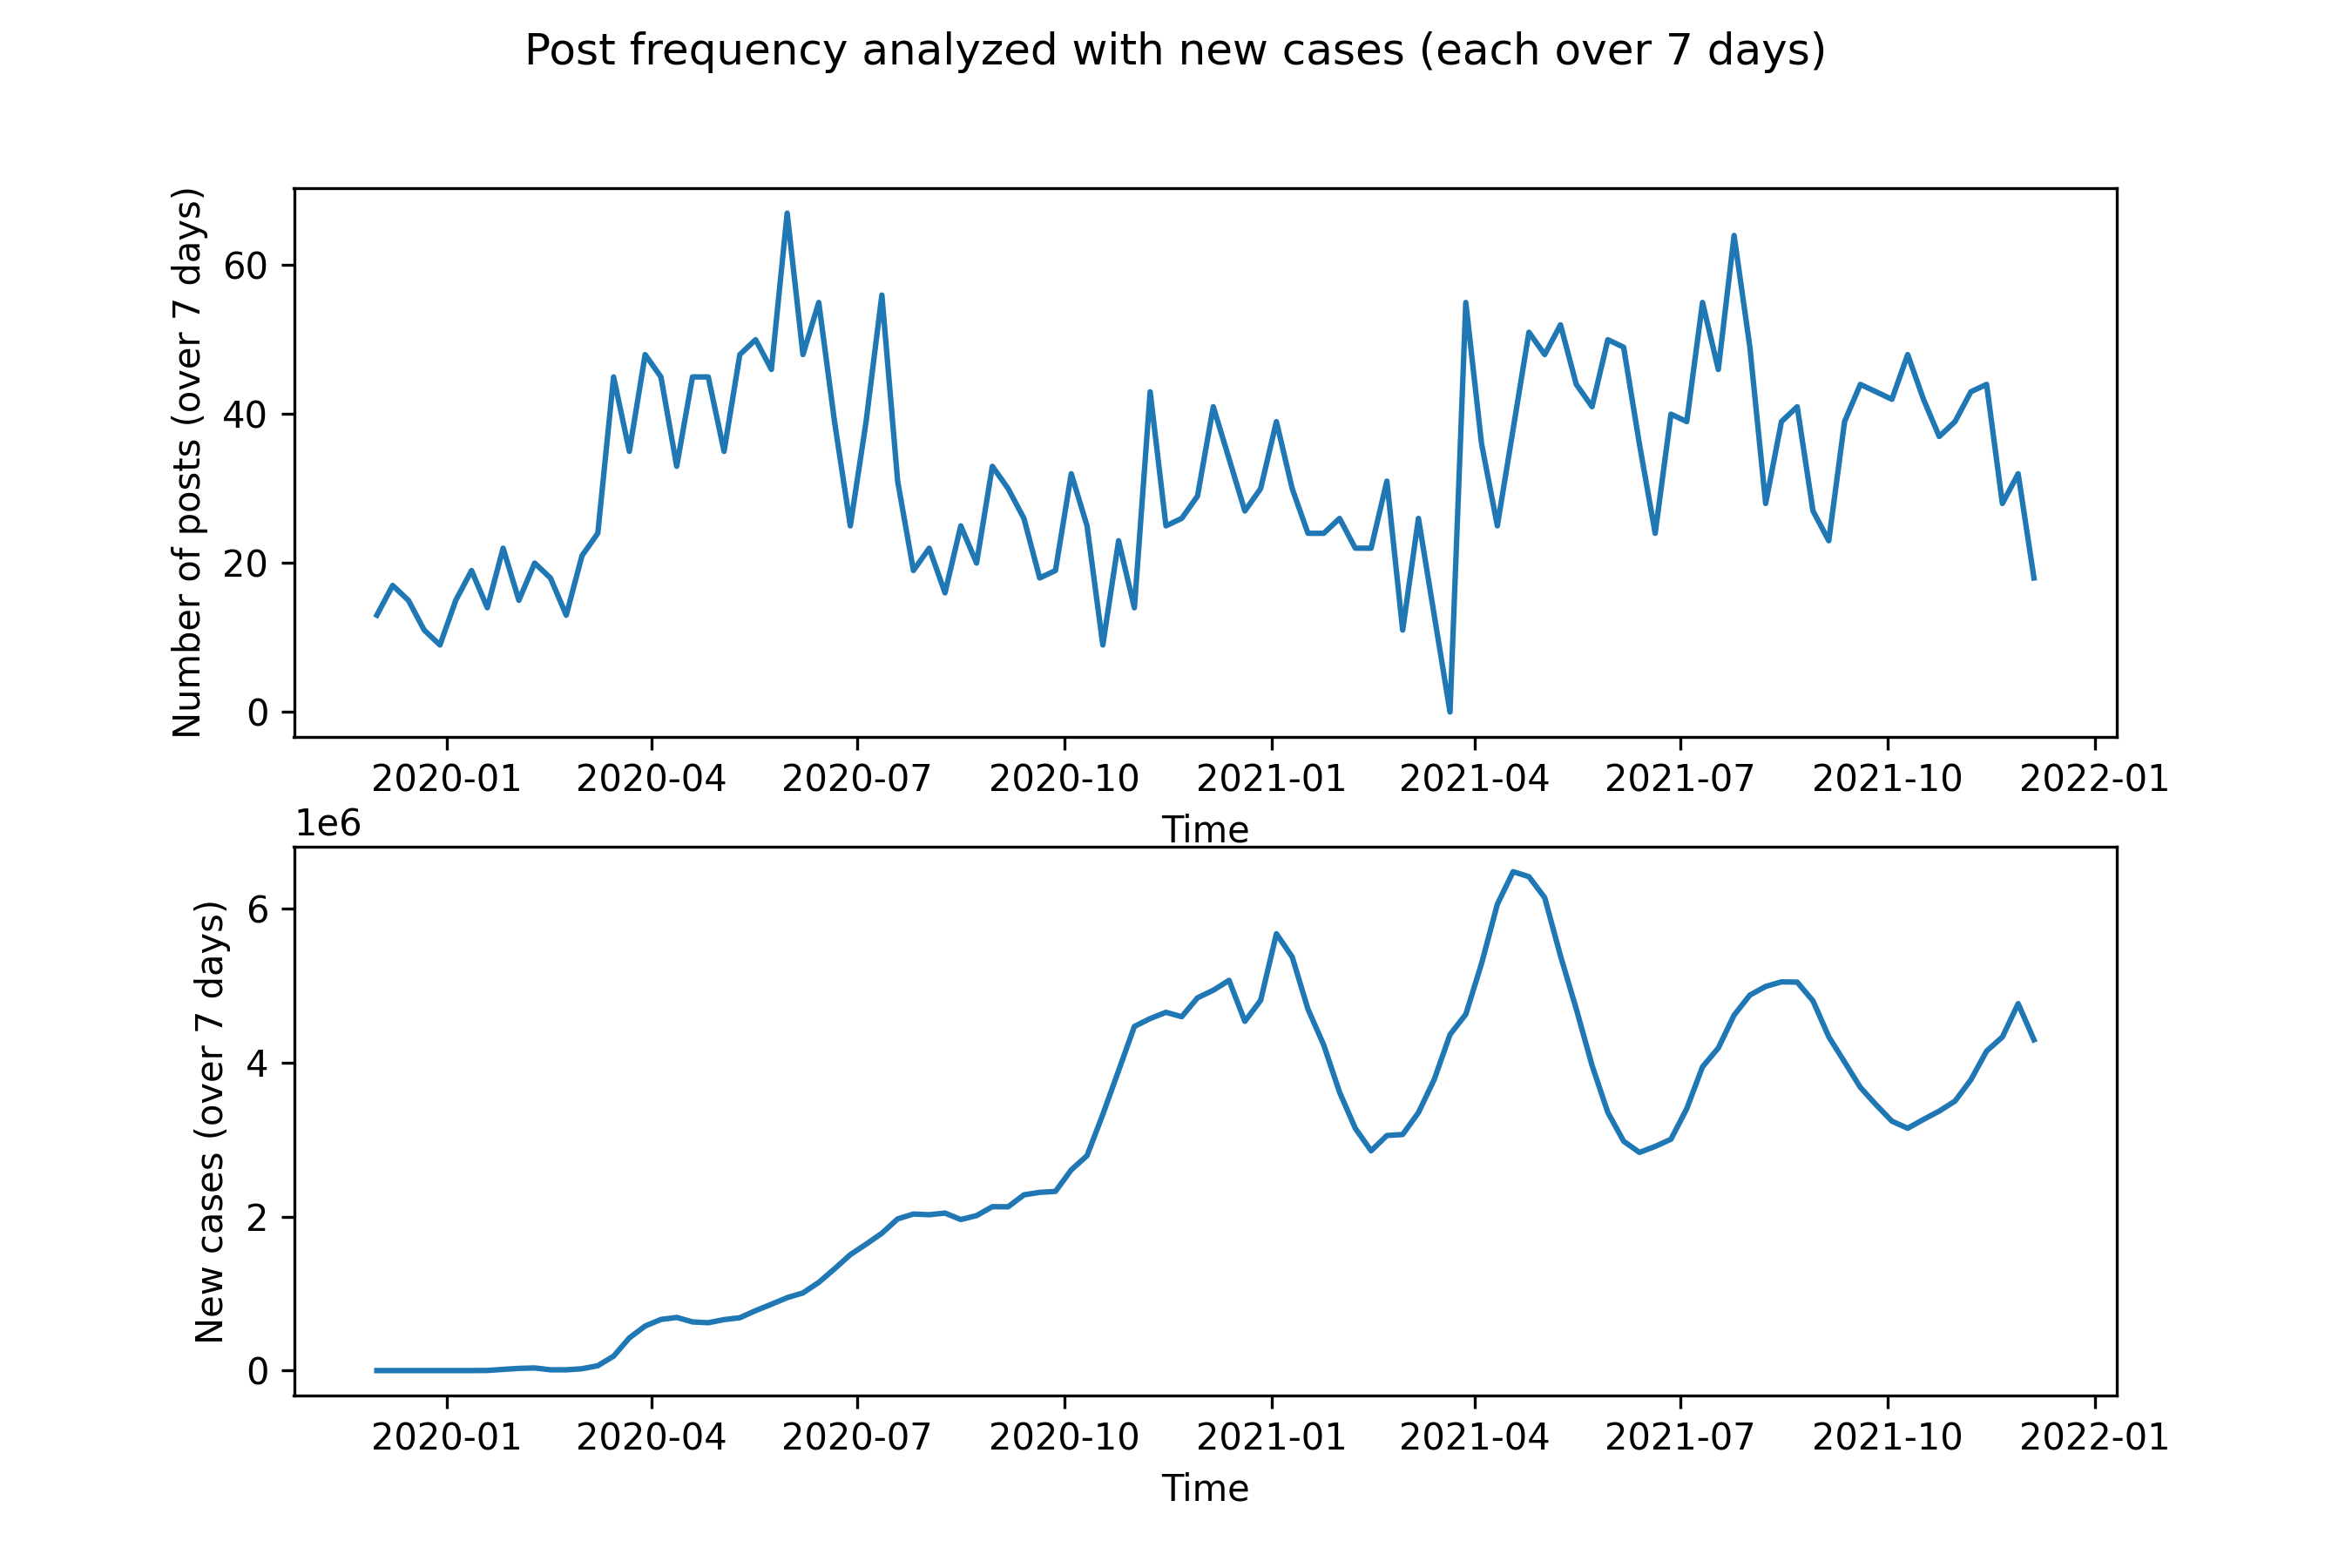
\includegraphics[width=14cm]{figures/frequency_over_time.png}
        \caption{\texttt{figures/frequency\_over\_time.png}}
        
    \end{figure}
    
    We observe a chaotically oscillating post frequency-time curve , noticing that the points at which case frequencies are highest coincide with significant increases in post frequencies. However, this relationship is best characterized by looking specifically at topic-related posts, which is done below.
    
    \item Popularity of the topics `covid' and `vaccine' over time
    
    \begin{figure}[H]
        \centering
        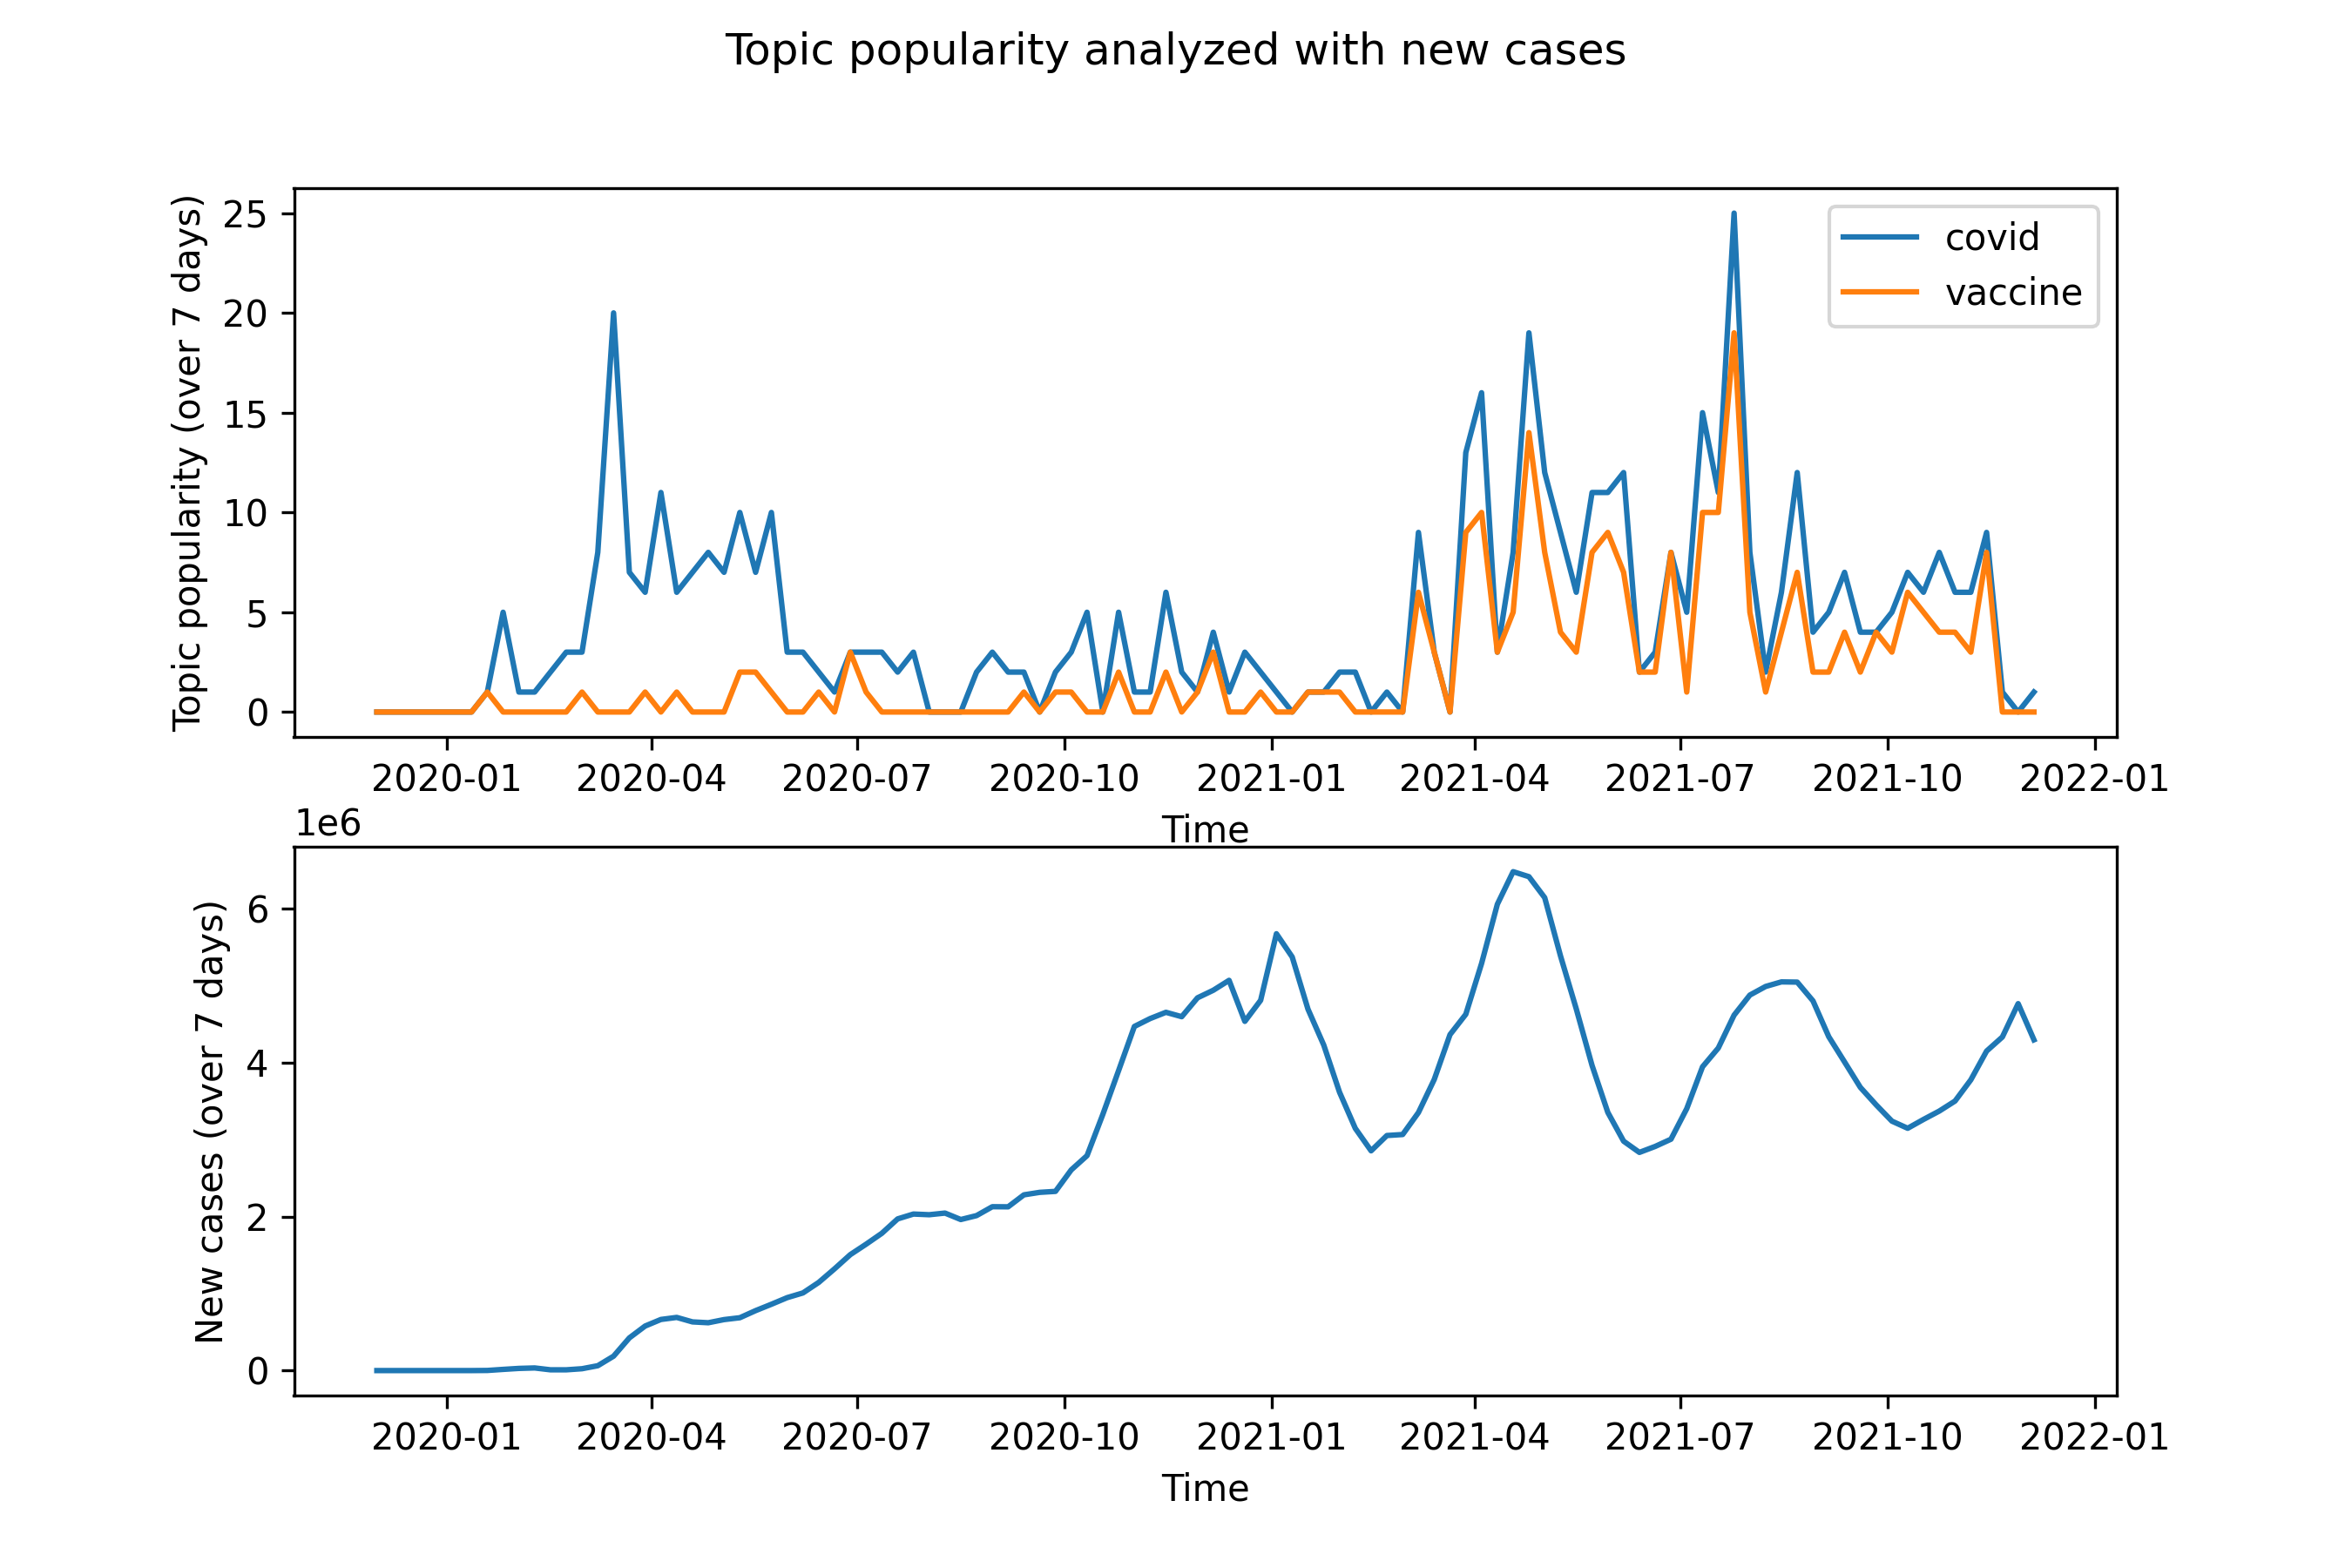
\includegraphics[width=14cm]{figures/popularities-covid-vaccine.png}
        \caption{\texttt{figures/popularities-covid-vaccine.png}}
        
    \end{figure}
        This figure makes it abundantly clear that the upticks in post frequencies around the times at which COVID-19 case frequencies were highest is attributable to COVID-related posts. It is also observed that COVID-19 is a very popular topic during the initial stages of the pandemic, and also that the nonexistence of a vaccine at that point of time yielded low popularities in the topic `vaccine'.


    
    \item Popularity of other topics over time
    
    \begin{figure}[H]
        \centering
        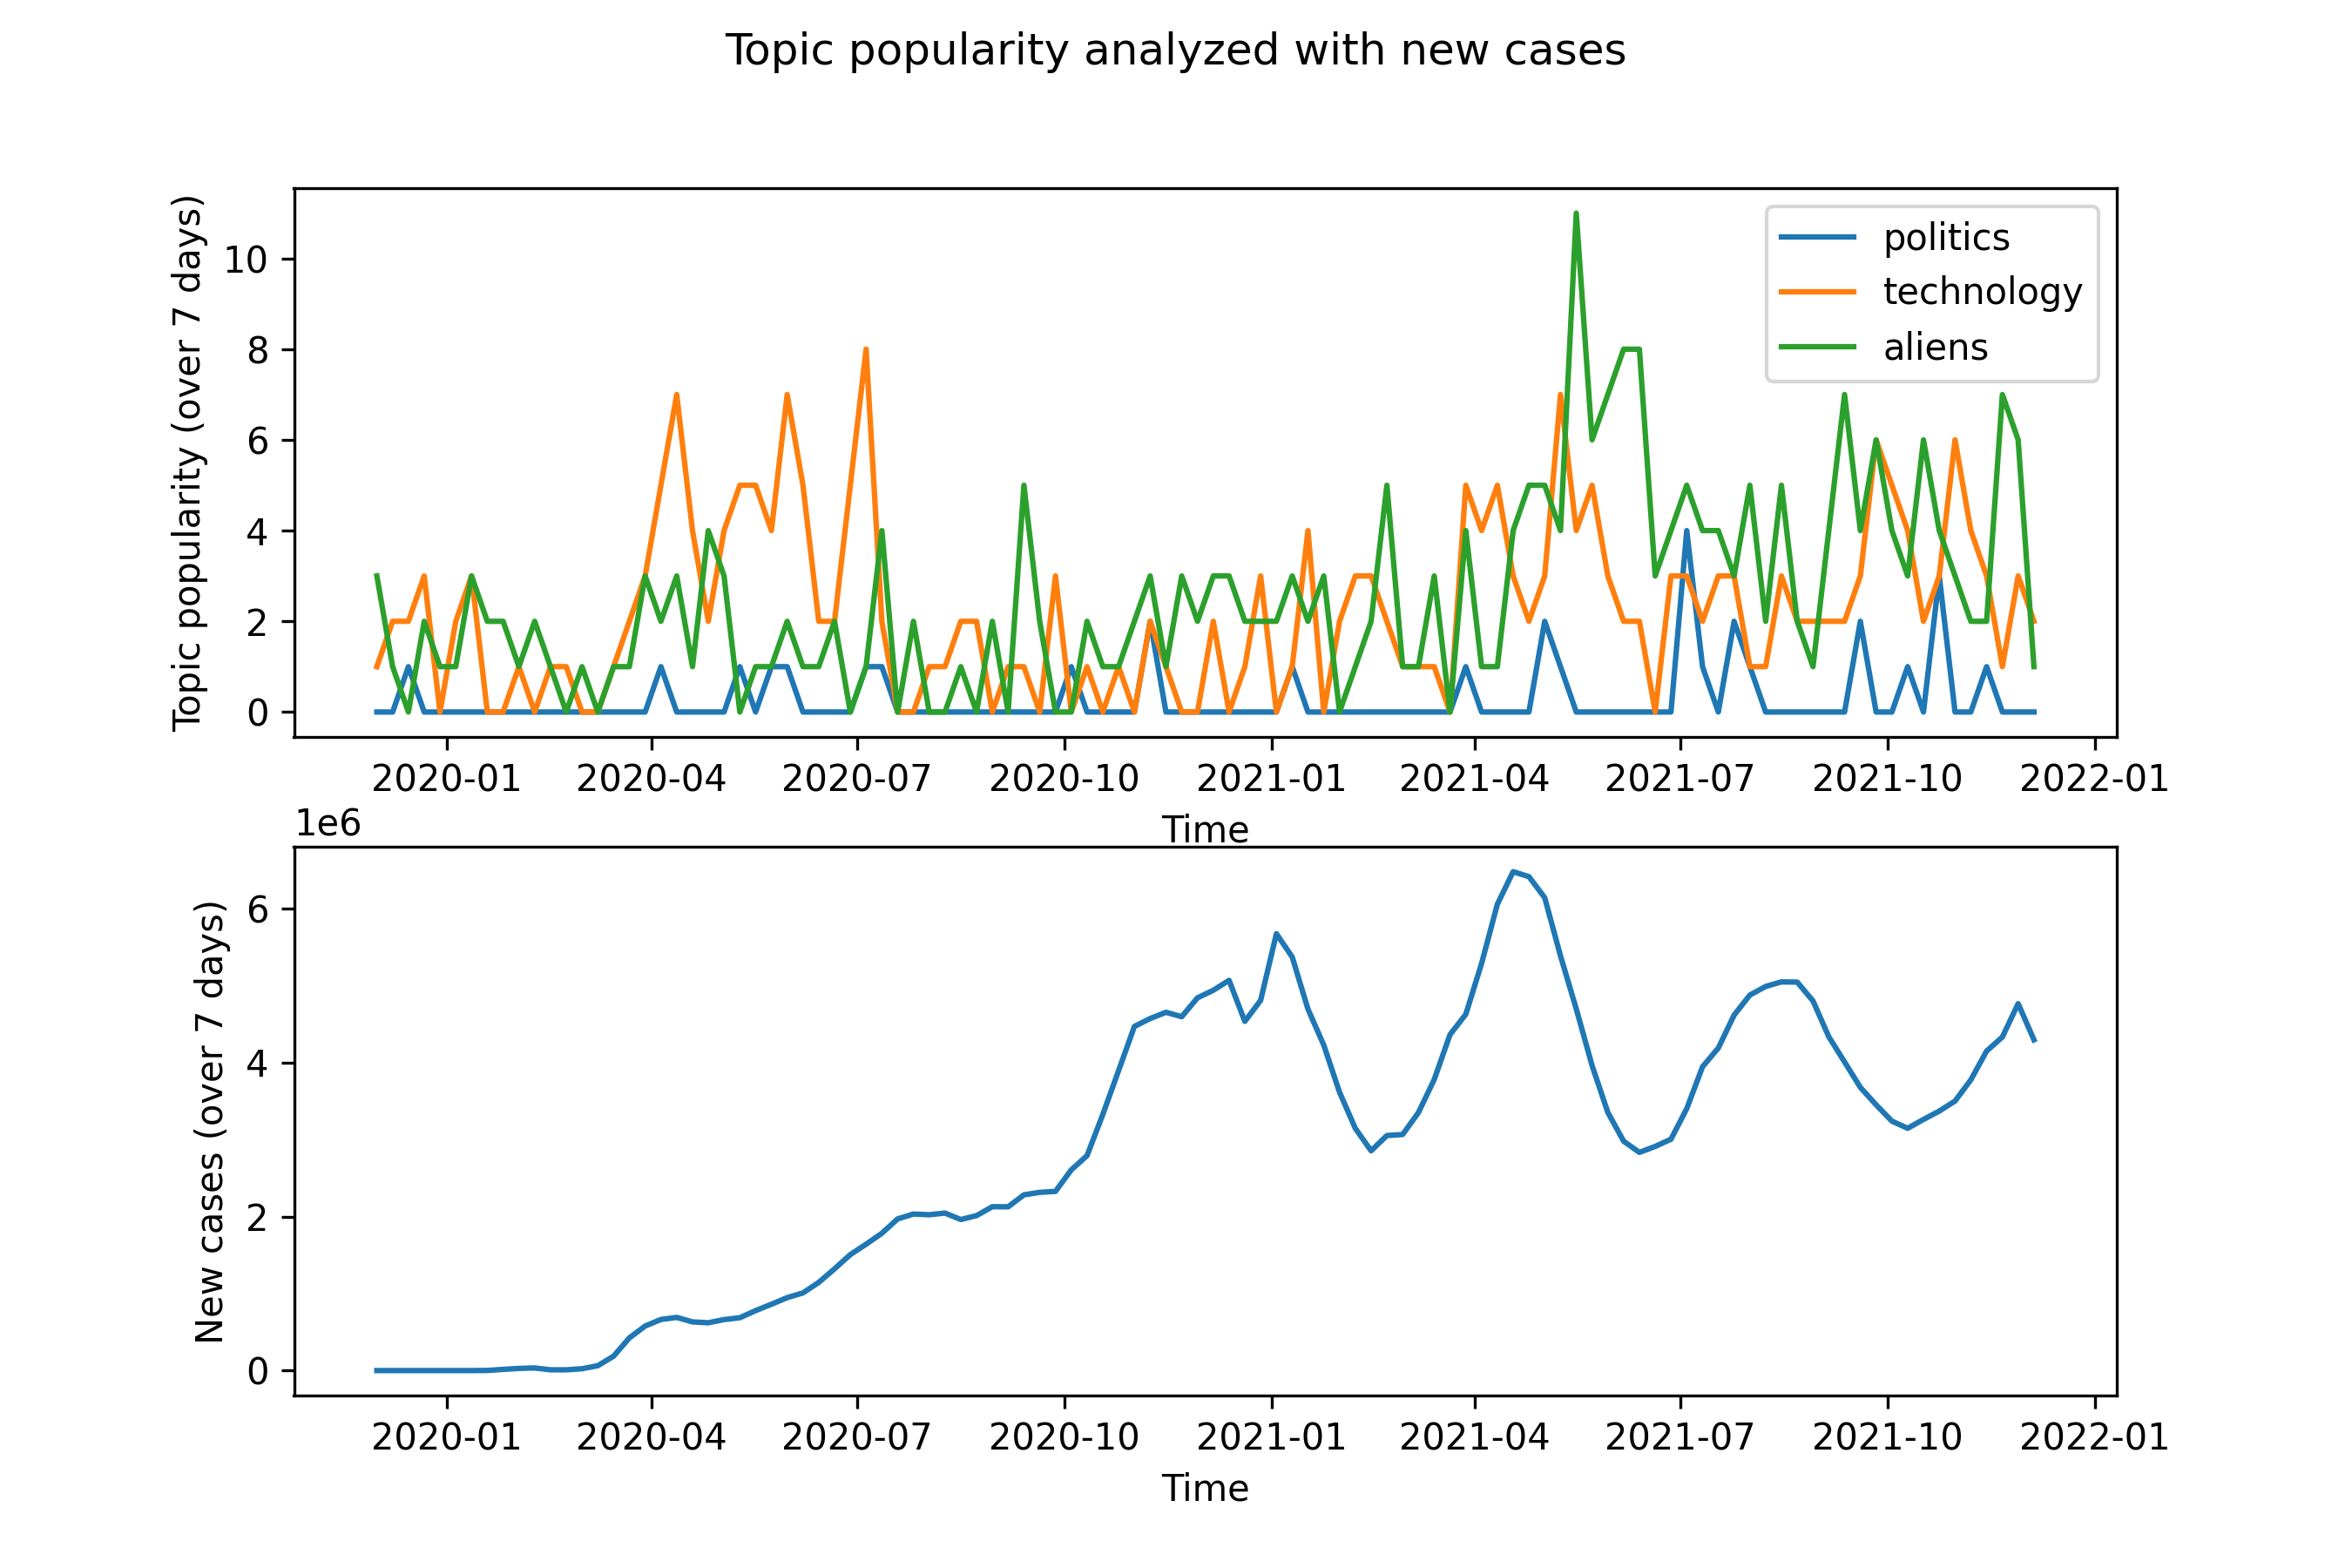
\includegraphics[width=14cm]{figures/popularities-politics-technology-aliens.png}
        \caption{\texttt{figures/popularities-politics-technology-aliens.png}}
    \end{figure}
    
    
    
    \item Total valence per week over time
    
    \begin{figure}[H]
        \centering
        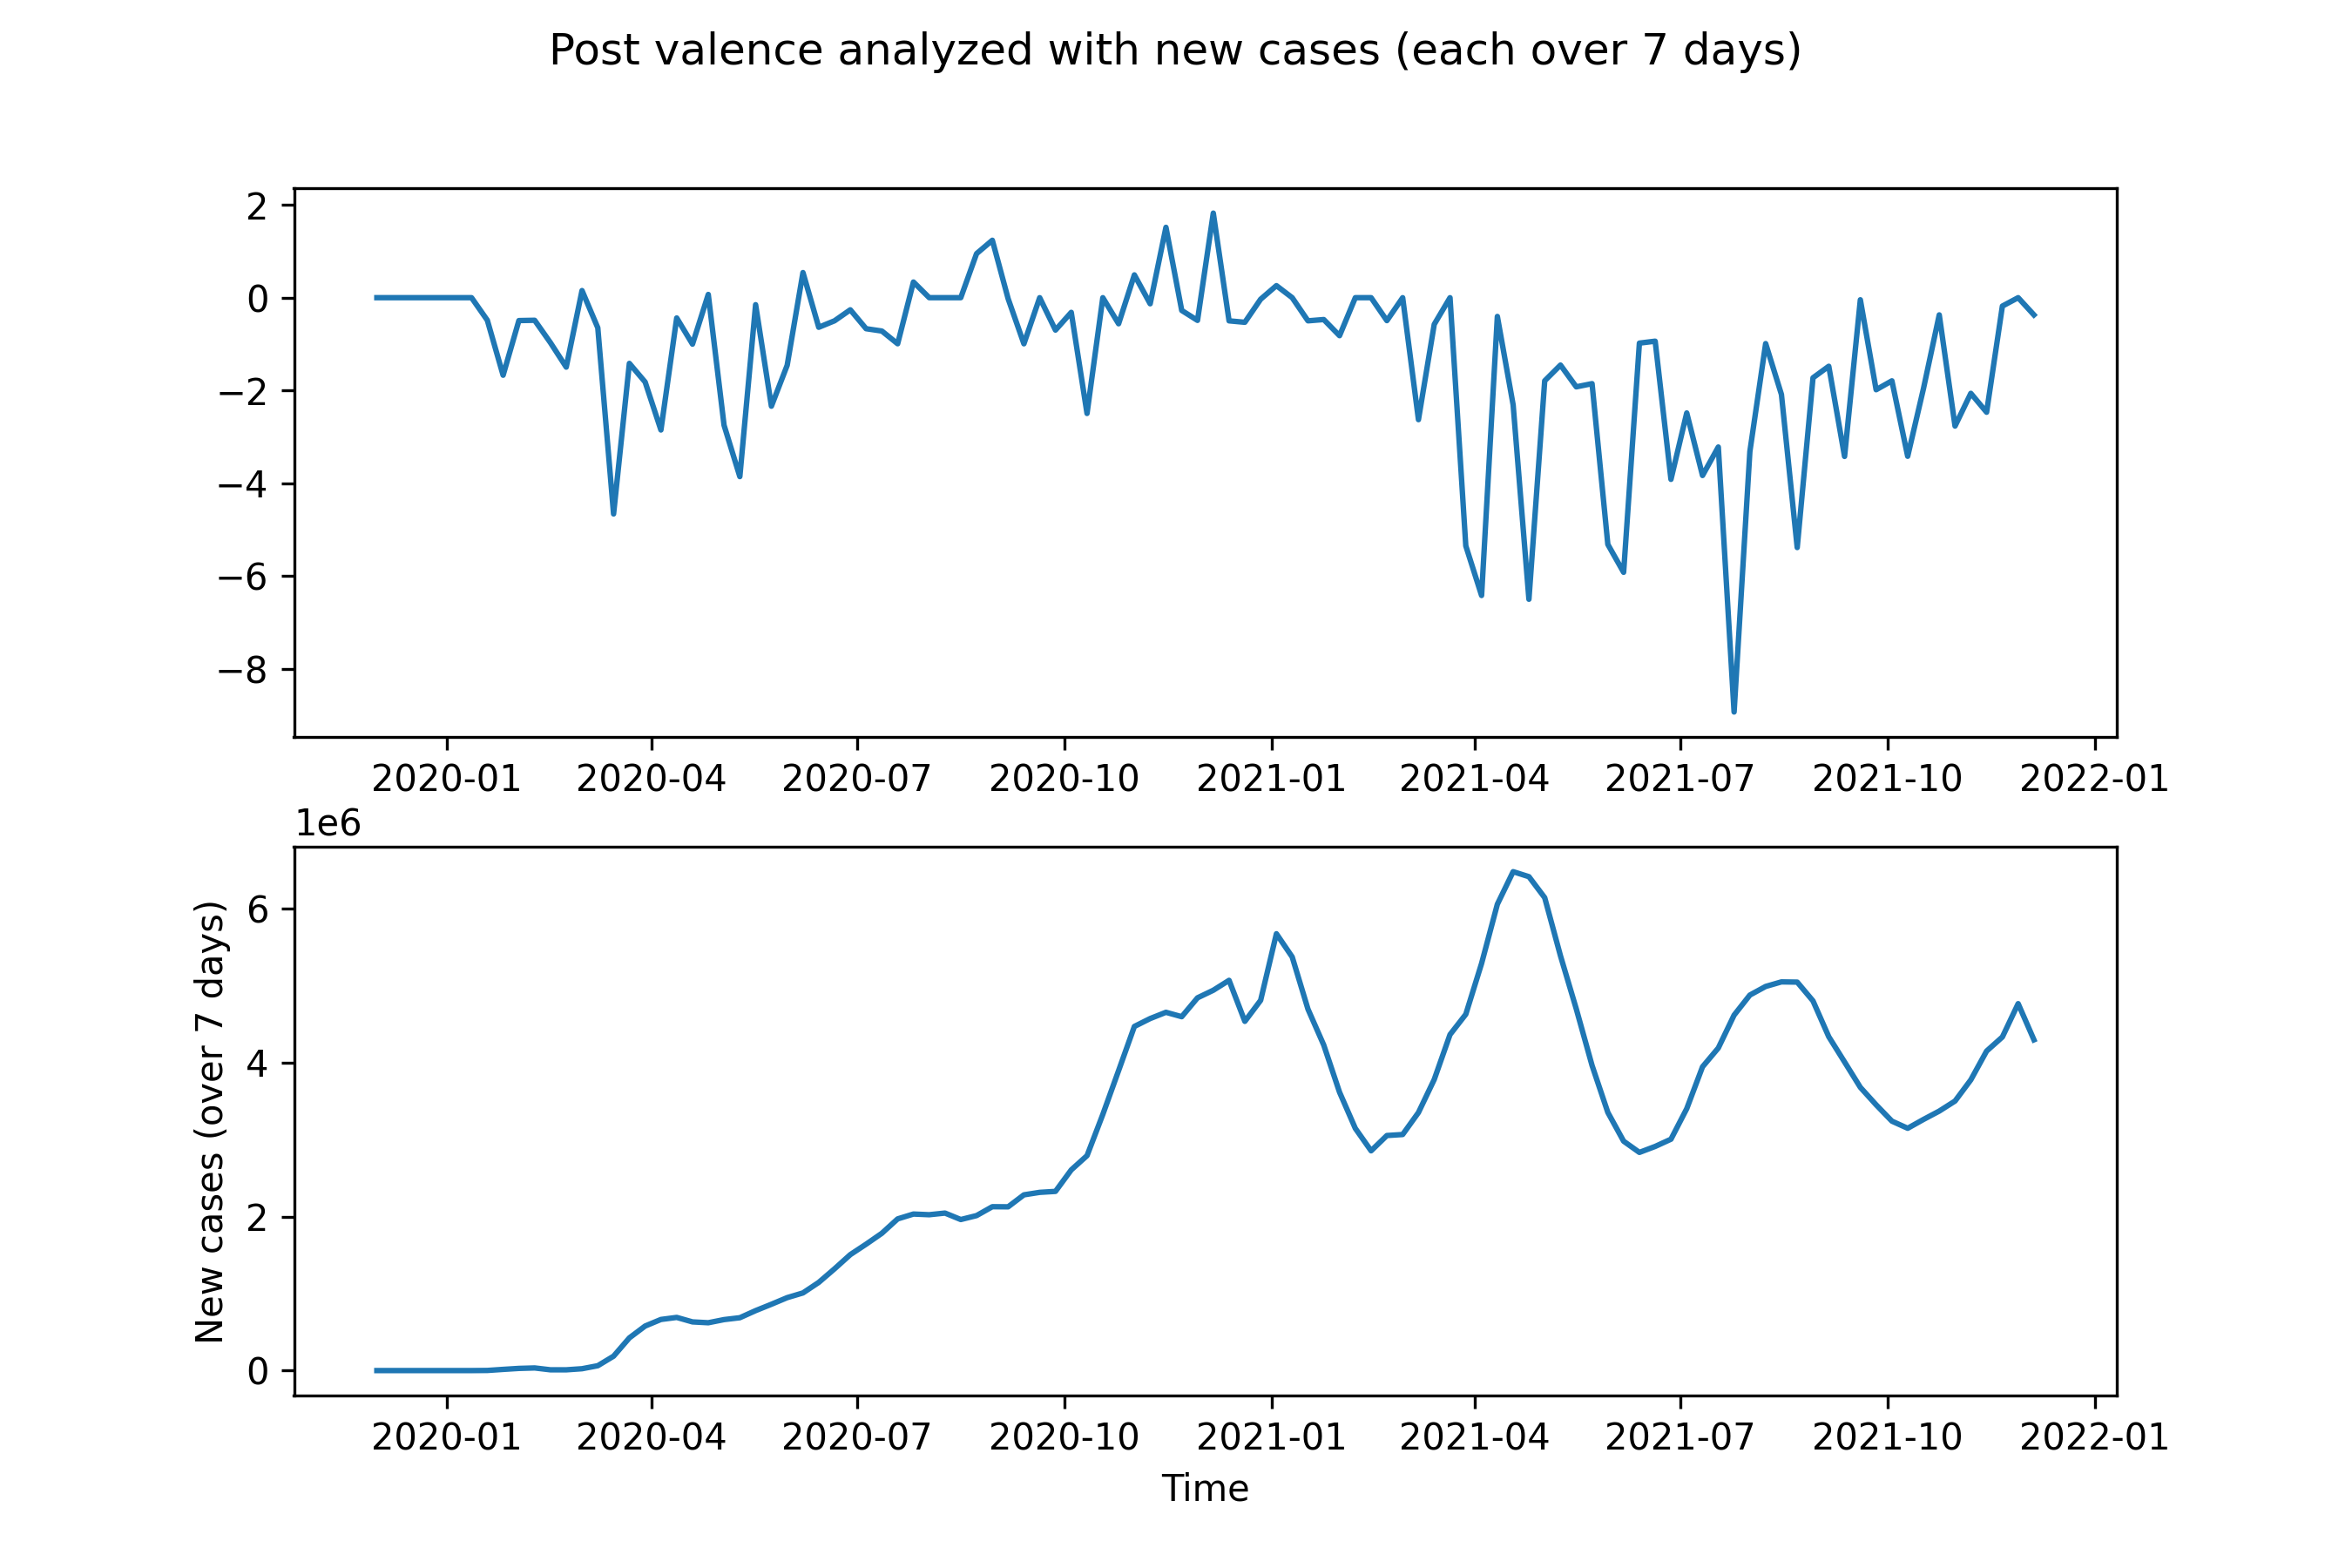
\includegraphics[width=14cm]{figures/valence_over_time.png}
        \caption{\texttt{figures/valence\_over\_time.png}}
        
    \end{figure}
    
    One of the most significant indicators is the large drop in total post valence around the time of the third rise in case frequencies around July 2021. This fall in net valence shows that in addition to the number of posts being high, the vast majority of them were negatively charged.
    
    \item Distribution of valences
    
    \begin{figure}[H]
        \centering
        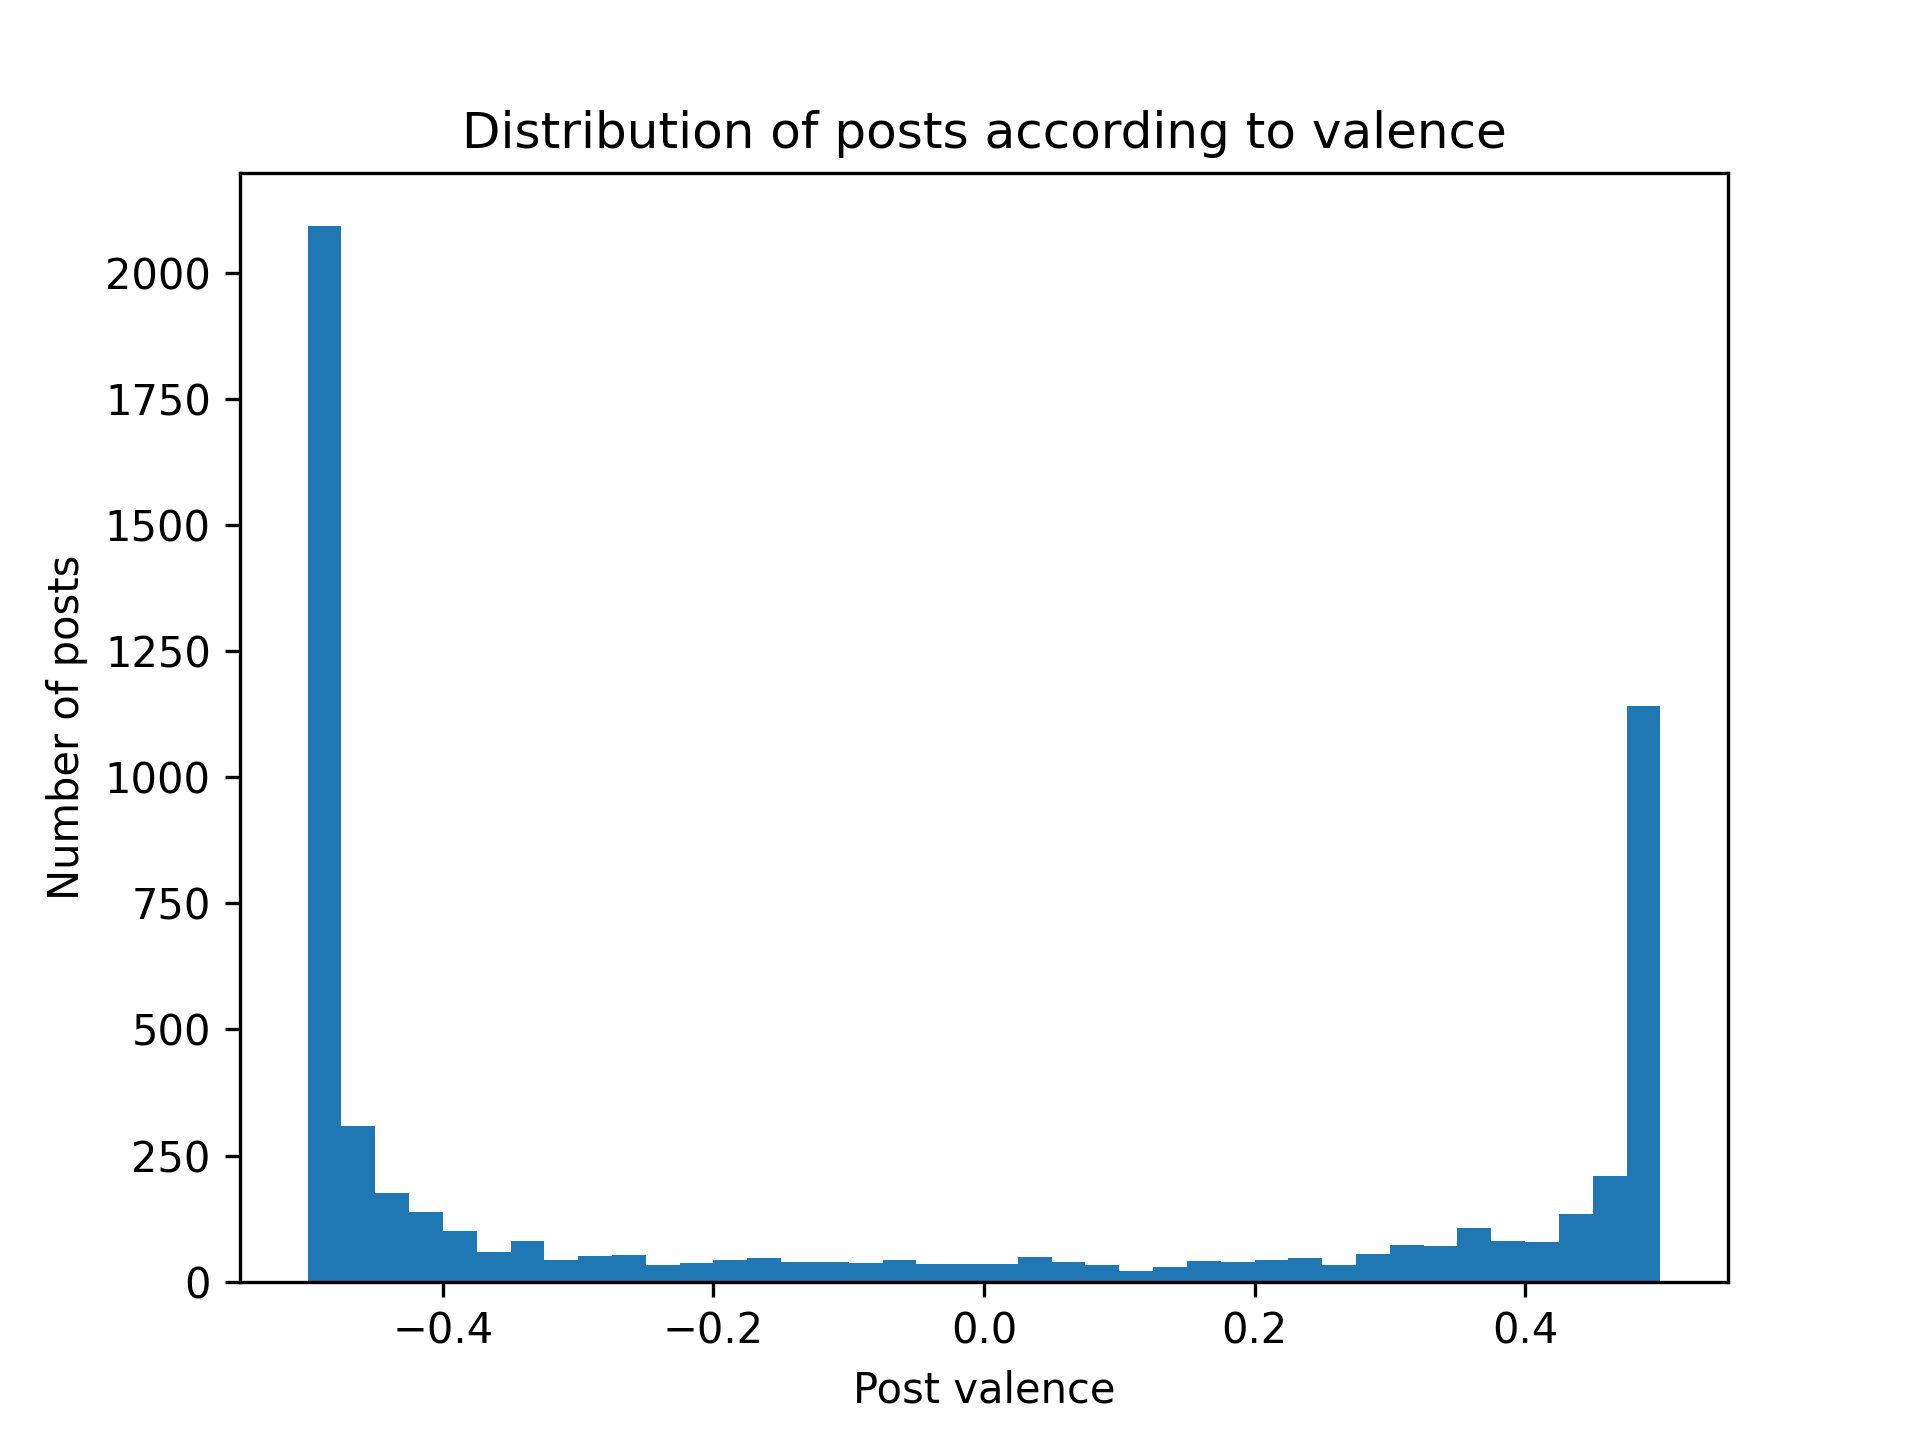
\includegraphics[width=14cm]{figures/valence_histogram.png}
        \caption{\texttt{figures/valence\_histogram.png}}
    \end{figure}
    
    This figure allows us to build upon the inferences we made from the previous one; indeed, we see that most posts are negative. More than anything else, this figure suggests that the majority of posts lie on the extreme ends of the negativity/positivity spectrum.
    
    \item Popularity of posts vs valences 
    
    \begin{figure}[H]
        \centering
        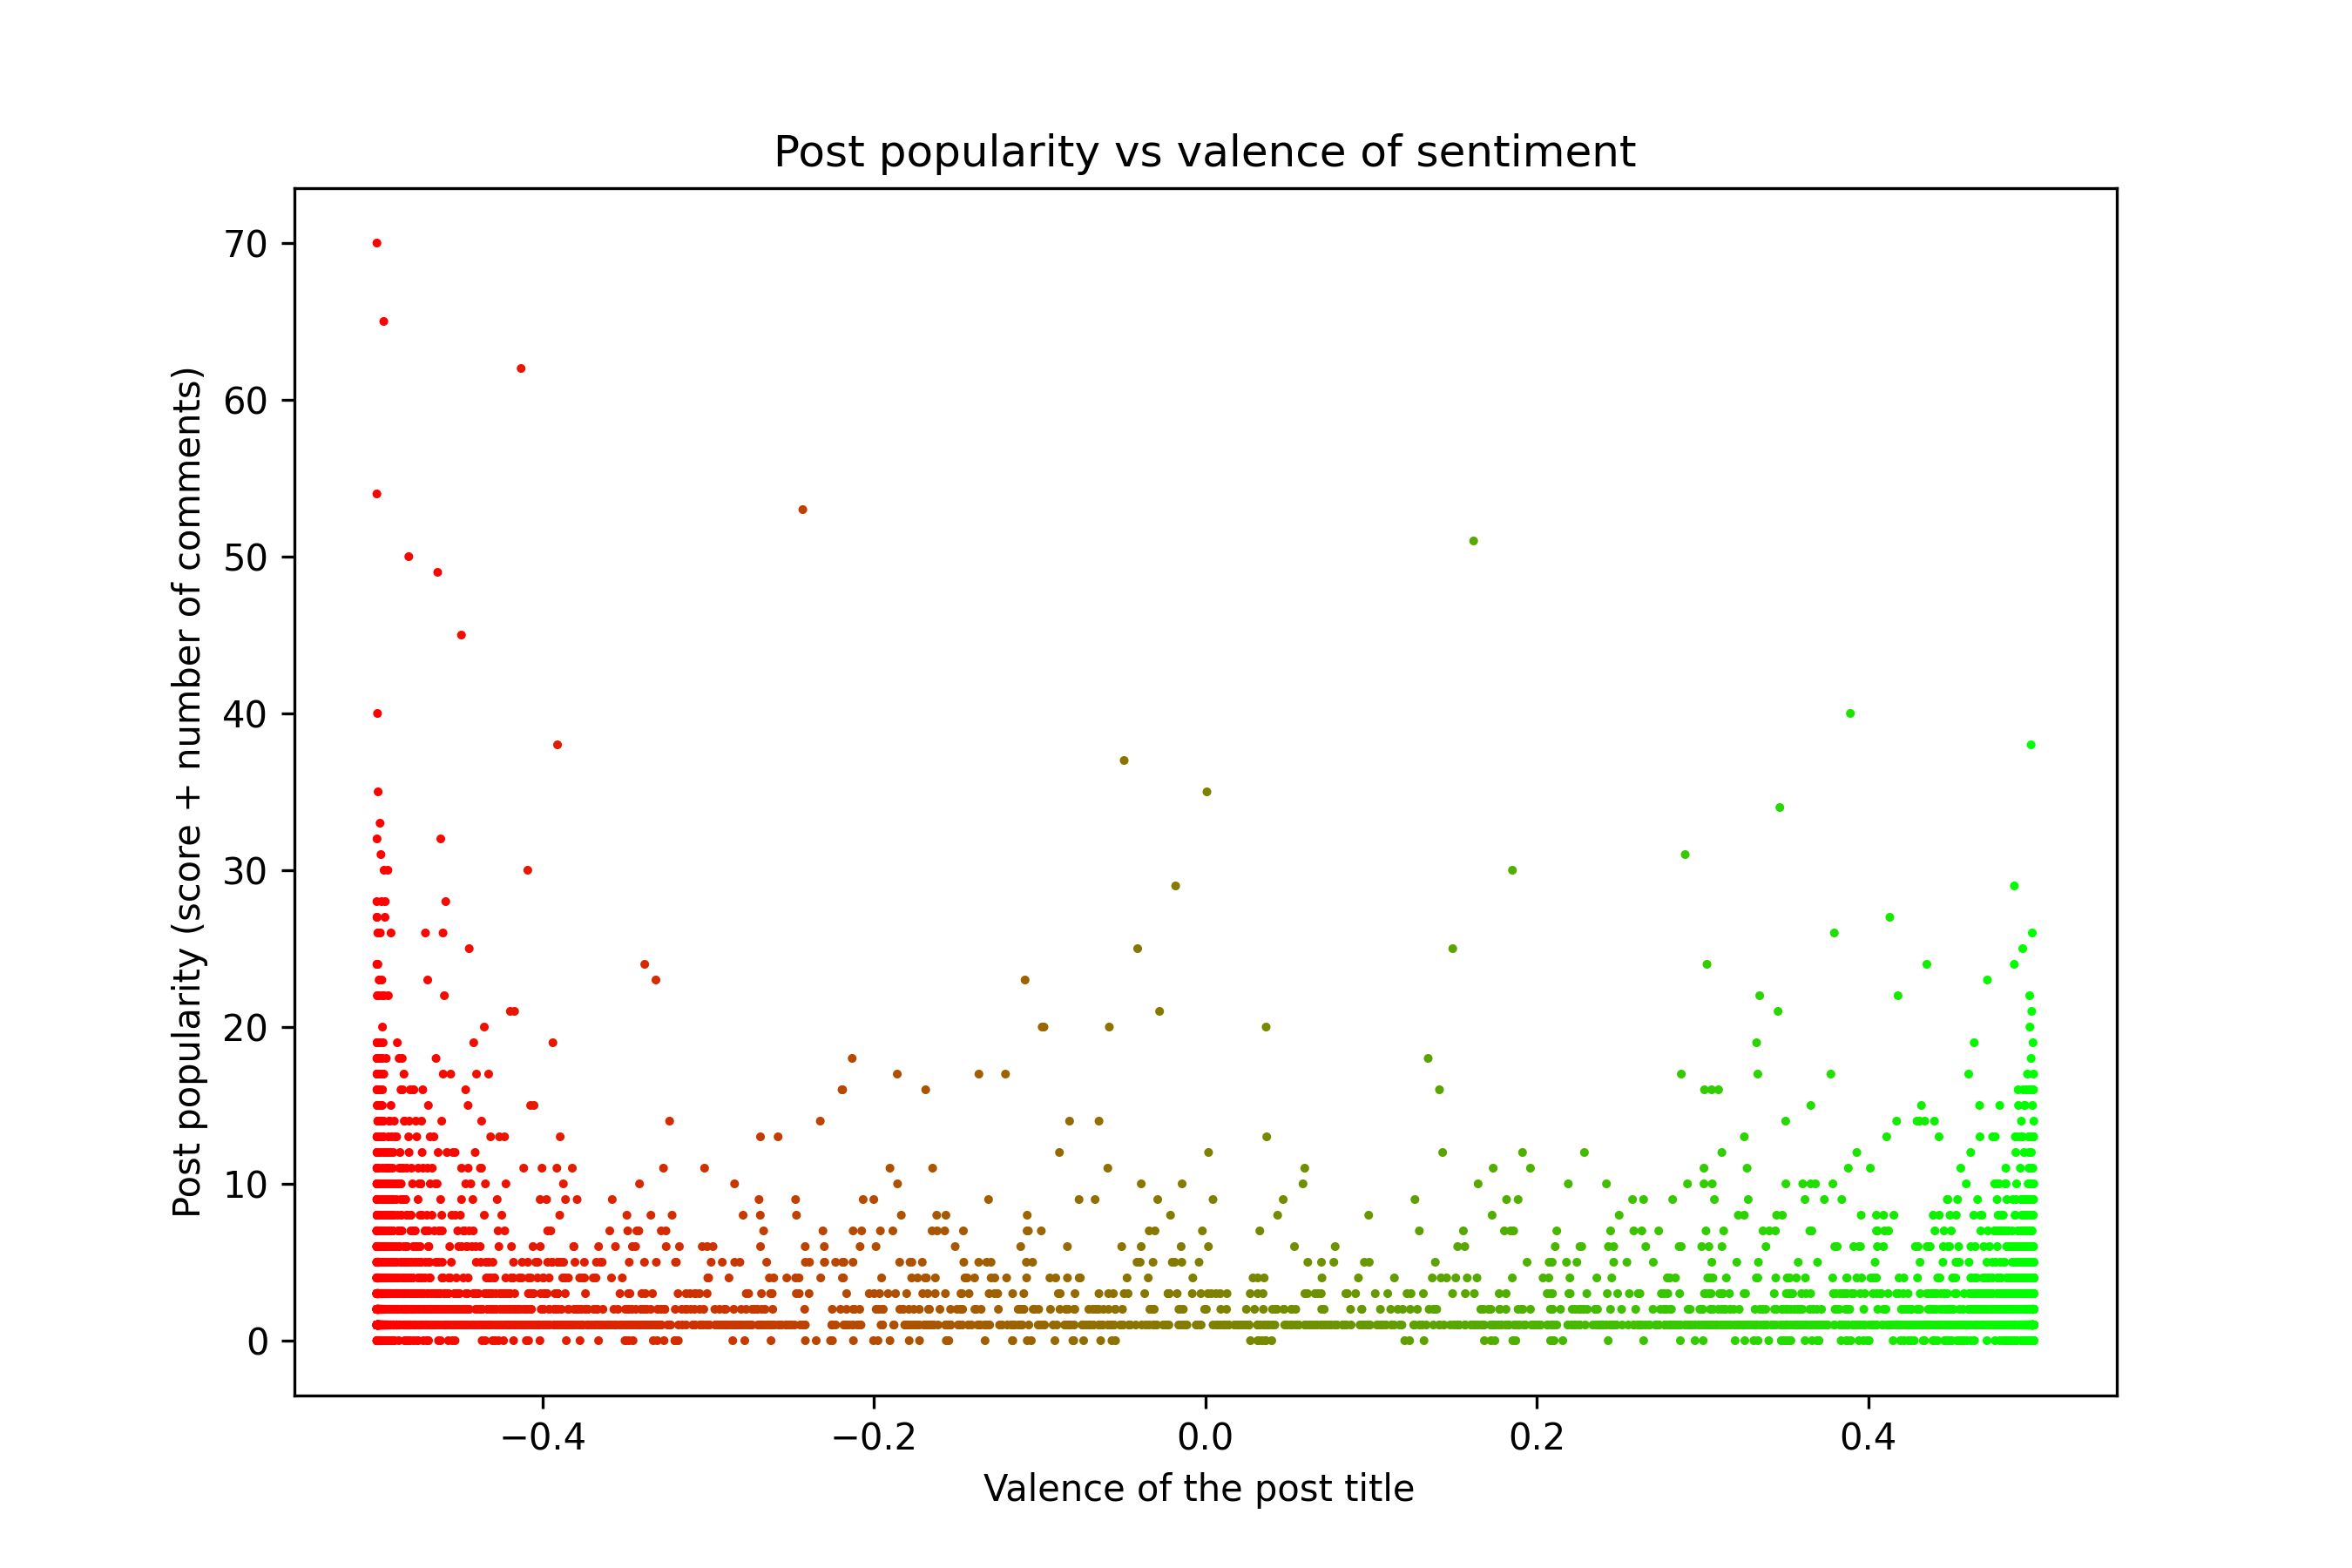
\includegraphics[width=14cm]{figures/sentiments_popularity.png}
        \caption{\texttt{figures/sentiments\_popularity.png}}
    \end{figure}
    
    Here, we observe that posts on the extremes of negativity/positivity tend to have the greatest popularity, with the extremely negative posts being  more popular and frequent in popularity than the extremely positive posts.
    
\end{enumerate}


Returning to our research question, we may now begin to develop plausible explanations for the trends observed in the above results.

\subsection{Addressing the Research Question}

Our research question was \textbf{What is the nature of the circulation and development of conspiracy theories surrounding COVID-19?}

From the above discussion, we can conclude the following: 

\begin{itemize}
    \item COVID-19 conspiracy theories are discussed with the greatest frequency during the beginning of the pandemic in early 2020, and the two major waves in April and August 2021. This early spike can likely be attributed to the novelty of the coronavirus subject.
    \item After March 2021, the time around which the vaccine roll-out began to take shape, vaccines are discussed in these theories very similarly in frequency to COVID-19 conspiracy theories.
    \item Posts which are either very positive or very negative tend to do well; posts which are very negative have the largest popularity.
\end{itemize}

The next spike in covid-related conspiracy posts happened around the start of 2021. This happened along with a large amount of vaccine related posts being made. Therefore, it is likely that these posts were made in response to the possibility of a covid vaccine being administered. 

\subsection{Limitations}
Our analysis was limited by the following :
\begin{itemize}
    \item We only linked topics to posts in a discrete manner when we could have used a more advanced intent detection algorithm to analyze the topic of each post.
    \item We did not analyze comment data on the posts which were processed - this could greatly aid in assessing the valence of a post and computing an overall compound popularity.
    \item Our list of keywords was large, but not exhaustive.
\end{itemize}

\subsection{Further work}

The following further work is suggested:

\begin{itemize}
    \item Develop a more sophisticated algorithm that determines a more precise degree (ie. floats between 0 and 1) of relation between topics and posts.
    \item Incorporate comment data into our analysis.
    \item Incorporate more subreddits into our analysis.
    \item Compile a larger list of keywords.
\end{itemize}

\printbibliography

\end{document}